\chapter{Evaluation}
\label{sec:evaluation}

In this section, we explore a single
high-level question: is Sieve practical?
To answer this question, we integrate
Sieve with Open mHealth~\cite{omh}, an
open source web service that allows users
to analyze their health data. We demonstrate
that the integration is straightforward, and
that the end-to-end application pipeline can
handle realistic workloads. Using
microbenchmarks, we also demonstrate that
Sieve's optimizations for avoiding costly
ABE operations (\S\ref{sec:minAbeCost})
are crucial for making Sieve practical.

\begin{figure*}
\centering
  \subfloat[Encryption speed: ABE and Ed448 in randomized counter mode.]{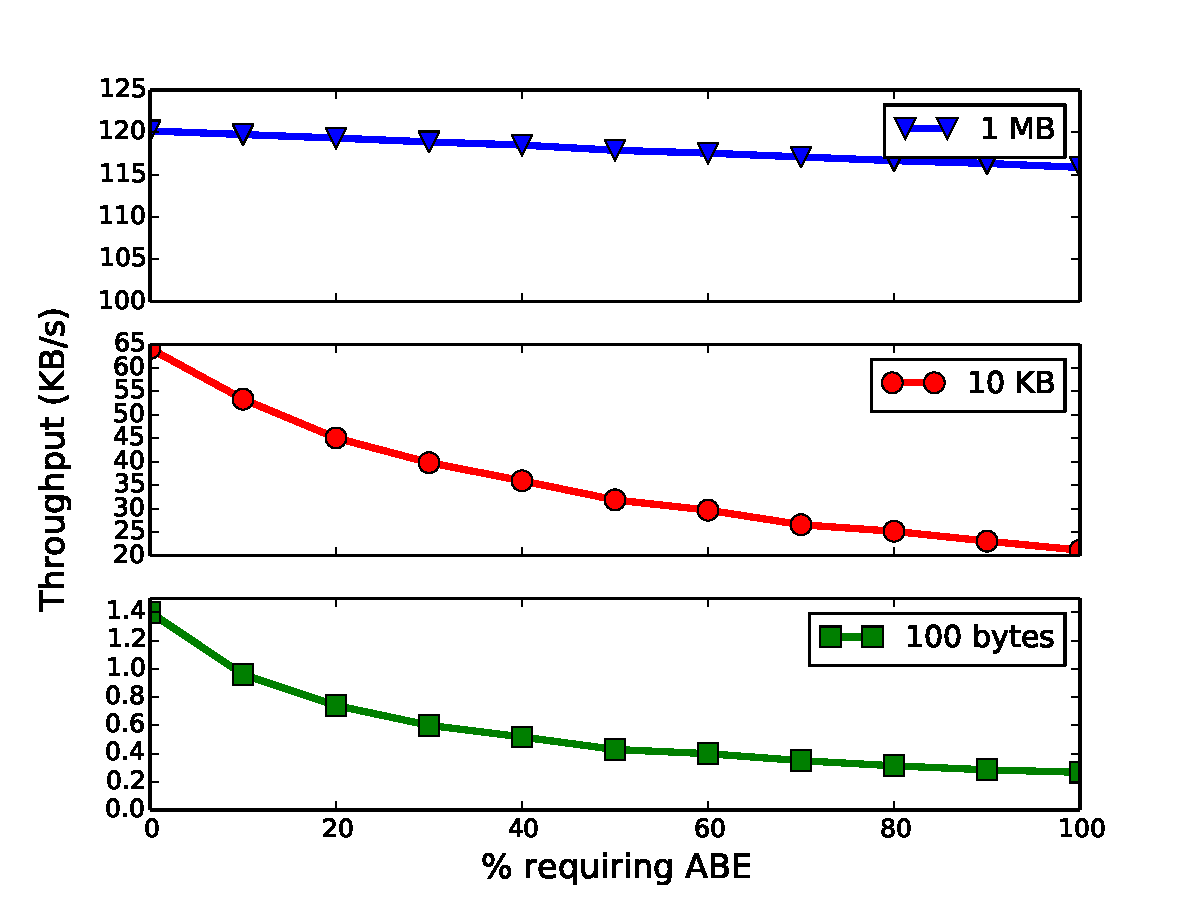
\includegraphics[width=0.48\textwidth]{figs/throughput1.pdf}\label{fig:throughput_ec}}
  \subfloat[Encryption speed: ABE and AES in CTR mode.]{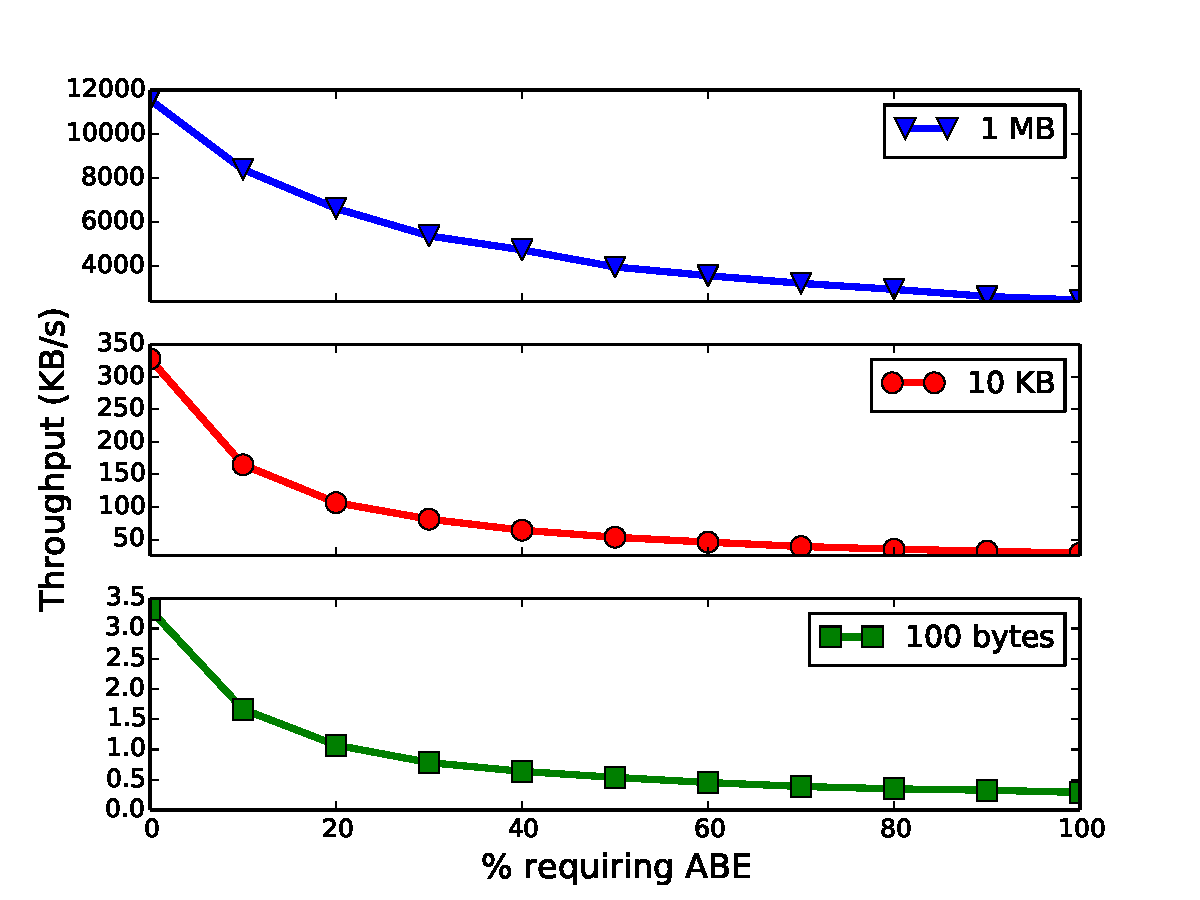
\includegraphics[width=0.48\textwidth]{figs/throughput2.pdf}\label{fig:throughput_aes}}
    \caption[ABE throughputs for Sieve]{Encryption throughputs for Sieve, as a function of 1) the size of
             the data to symmetrically encrypt, 2) the percentage of symmetric
             data encryptions which also require the ABE encryption of a
             metadata block, and 3) whether the cipher is AES or
             key homomorphic Ed448. All experiments assume that each metadata
             block has five attributes, and each ABE key has 10. Performance
             trends for decryption are similar.}
\label{fig:throughput}
\end{figure*}

All experiments ran on a machine with a 2 GHz
Intel Core i7 and 8 GB of RAM. We ran each
experiment 50 times, and we report the average
(standard deviations were small).
%{\bf !!!jwm: Can we say how small?}
Sieve used 2048 bit RSA with SHA256 to sign
user objects. To symmetrically encrypt those
objects, Sieve used 128-bit AES in CTR mode,
or Ed448-Goldilocks elliptic curves in randomized
counter mode; the latter cipher is key
homomorphic (\S\ref{sec:revocation}), but the
former is not. ABE operations used 224-bit MNT
curves~\cite{mnt224}. All web servers ran on the test
machine's loopback interface, to minimize
network latency and focus on Sieve's cryptographic
overheads.

All GUIDs were 64 bits long. Thus, a metadata
block which contained a GUID and an AES key
was 24 bytes in size, whereas a metadata block
with a GUID and an Ed448 key was 64 bytes long.

\section{Integrating Sieve with Open mHealth}
\label{sec:integration}
Open mHealth allows users to upload medical
data to a web server that will analyze the
data and provide explanatory visualizations.
To integrate Sieve with Open mHealth, we first 
forced the Open mHealth
client to upload data via the Sieve client
instead of directly to the Open mHealth server.
We then ran a Sieve import daemon on the Open
mHealth web server, configuring the daemon
with the data schema that the Open mHealth
analytics engine uses. These modifications
required approximately 200 lines of code
to be changed in the Open mHealth platform.

To test the end-to-end performance of the
application pipeline, we used Open mHealth's
data generator to create a week's worth of
health data. The data included information
like weight, blood pressure, physical activity,
and heart rate. Each day had approximately
14 data points. For each data point, the
Sieve client added attributes like the
date that the sample was collected, the
name of the associated user, and the type
of data represented by the sample. The Sieve
client used a single storage-based data 
structure to store the samples for an entire week.

The cost to upload the first data point
at the beginning of a week was 1.1 seconds;
the cost was dominated by ABE encryption.
Uploading subsequent data points proceeded
at the throughput of the symmetric cipher,
requiring 17.1 ms per data point for AES,
and 38.5 ms for Ed448.

On the server-side, importing an entire
week of data required 1.4 seconds for both AES 
and Ed448 if the server had not cached GUIDs or symmetric
keys; ABE decryption dominated the cost. 
In that scenario, the server had to
download the metadata block, decrypt it with
ABE, download the raw data block, and then
decrypt that block using a symmetric cipher. 
If the server cached GUIDs and symmetric keys,
accessing the entire week's data cost 0.08 seconds
with AES, and 0.75 seconds with Ed448.

\section{Microbenchmarks}
\subsection{Encryption speed} Sieve requires
clients to symmetrically encrypt each data
object before uploading it. Some fraction of
uploads will also require clients to ABE-encrypt
a metadata block. Minimizing that fraction
is important, because ABE operations are much
slower than symmetric operations. Figure~\ref{fig:throughput}
quantifies the performance gaps between ABE
and symmetric ciphers. For 10 KB objects,
pure ABE encryption throughput is 1.1 KB/s,
whereas pure Ed448 throughput is 23.8 KB/s
and pure AES throughput is 43.5 KB/s.
Although clients can perform data uploads
asynchronously, in the background, the
computational costs for ABE are still quite
high. Thus, the optimizations from
Section~\ref{sec:minAbeCost} are crucial
for minimizing the number of ABE operations.

Note that Ed448~\cite{ed448} is a new elliptic curve.
Implementations of symmetric ciphers using Ed448 
are currently slower than popular AES libraries,
but we expect Ed448's performance to improve as
its implementations mature.

\begin{figure}
\centering
\begin{tabular}{ |p{5.5cm}|p{1.5cm}| }
\hline
Operation & Time (s)\\ \hline
Generating 10 attribute key &  0.46\\ \hline
Generating 20 attribute key & 0.64\\ \hline
Re-encrypting a metadata block (10 attributes) & 0.63 \\ \hline
Re-encrypting a metadata block (20 attributes) & 0.91 \\ \hline
Re-key 100 KB data block & 0.41 \\ \hline
\end{tabular}
\caption{Computational overheads for key generation and revocation.}
\label{fig:sievekey}
\end{figure}

\subsection{Key generation and revocation}
Figure~\ref{fig:sievekey} describes the costs
that Sieve pays for generating new ABE keys,
re-encrypting metadata blocks, and re-keying
a 100 KB data block. The creation of new ABE
keys is rare, and only occurs when a new service
requests access permissions, or an old service
receives modified permissions (possibly as the
result of an epoch number increasing after a
revocation (\S\ref{sec:revocation}). During
revocation, the metadata blocks asssociated
with the revoked ABE key must be re-encrypted;
however, those metadata blocks will typically
point to a much larger number of raw data
blocks (\S\ref{sec:minAbeCost}), so the overall
re-encryption cost of revocation is governed
by the speed with which raw data can be re-keyed.

\subsection{Attribute matching} When the storage
provider receives a data access request from a
third party, the storage provider must locate
the metadata blocks whose attributes match those
of the access request. Sieve makes the matching
process fast by storing metadata blocks in a
database and indexing those blocks using their
attributes.

Due to space constraints, we omit a full description
of matching performance. However, the results
are unsurprising, since modern databases are good
at building indices. For example, in one experiment,
we injected 1 million metadata blocks into MongoDB;
each metadata block had 10 randomly selected attributes
from a universe of 35 possible attributes. Then, we
submitted access queries in which each query contained
5 random attributes joined with a random set of
\texttt{ANDs} and \texttt{ORs}. Each query took 1.1 ms
to complete.

\subsection{Secret-sharing} Sieve partitions the
ABE master key and the RSA signing key across
multiple devices, ensuring that a lost or stolen
device will not store a full copy of sensitive
cryptographic information. The secret sharing
protocol is cheap: ignoring network latencies,
and assuming that $k=2$ and $n=5$,
splitting a 2048 bit object like an RSA key
requires 0.04 ms, and reconstructing that key
requires 0.09 ms.
